\pagebreak
\section{Simulation Analysis}
\label{sec:simulation}

\indent

This section discusses the circuit simulation, performed using {\it Ngspice}. 

This circuit was entered into the {\it Ngspice} simulation environment. This tool is used to simulate analog electronic circuits and predict circuit behaviour. 
This {\it Ngspice} simulation begins by defining the reference node, which is the node with potential 0 (by convention). In {\it Ngspice}, this node is represented by $V_0$. In our theoretical analysis, the reference node was node 4. However node 4 is still needed because we must introduce a voltage source with 0V potential, in order to measure the current $I_c$ for the dependent voltage source, since {\it Ngspice} considers the voltage sources as Ammeters.
The new diagram, which represents more accurately what was introduced in {\it Ngspice}, is shown on Figure~\ref{fig:ngspiceCircuit}.

\begin{figure}[H] \centering
    \includegraphics[width=0.8\linewidth]{t2_ngspiceLabels.pdf}
    \caption{Voltage and Current driven circuit with 7 resistors.}
    \label{fig:ngspiceCircuit}
\end{figure}



\subsection{Circuit analysis for $t<0$}

\indent

Table \ref{tab:OpNg} shows the simulated operating point results for the circuit
under analysis when $t<0$, which means that the capacitor acts as an open circuit and therefore $I_c=0$.
\begin{table}[H]
  \centering
  \begin{tabular}{|l|r|}
    \hline    
    {\bf Name} & {\bf Value [A or V]} \\ \hline
    @c[i] & 0.000000e+00\\ \hline
@gcs[i] & -2.04136e-04\\ \hline
@r1[i] & 1.945229e-04\\ \hline
@r2[i] & -2.04136e-04\\ \hline
@r3[i] & -9.61363e-06\\ \hline
@r4[i] & 1.156284e-03\\ \hline
@r5[i] & 2.041365e-04\\ \hline
@r6[i] & 9.617613e-04\\ \hline
@r7[i] & 9.617613e-04\\ \hline
v(1) & 5.008942e+00\\ \hline
v(2) & 4.808960e+00\\ \hline
v(3) & 4.394159e+00\\ \hline
v(4) & 0.000000e+00\\ \hline
v(5) & 4.837862e+00\\ \hline
v(6) & 5.474755e+00\\ \hline
v(7) & -2.00872e+00\\ \hline
v(8) & -2.97092e+00\\ \hline

  \end{tabular}
  \caption{Operating point analysis. A variable preceded by @ is of type {\em current}
    and expressed in Ampere; other variables are of type {\it voltage} and expressed in
    Volt.}
  \label{tab:OpNg}
\end{table}


\subsection{Circuit analysis for a voltage source-equivalent capacitor}

\indent

Table \ref{tab:Op2Ng} shows the simulated operating point results for the circuit under analysis when the capacitor acts as a voltage source outputting: $V_X=V_6-V_8$ and the voltage source is turned off ($V_s=0$).
\begin{table}[H]
  \centering
  \begin{tabular}{|l|r|}
    \hline    
    {\bf Name} & {\bf Value [A or V]} \\ \hline
    @gcs[i] & -2.04136e-04\\ \hline
@r1[i] & 1.945229e-04\\ \hline
@r2[i] & -2.04136e-04\\ \hline
@r3[i] & -9.61363e-06\\ \hline
@r4[i] & 1.156284e-03\\ \hline
@r5[i] & 2.041359e-04\\ \hline
@r6[i] & 9.617613e-04\\ \hline
@r7[i] & 9.617613e-04\\ \hline
v(1) & 5.008942e+00\\ \hline
v(2) & 4.808960e+00\\ \hline
v(3) & 4.394159e+00\\ \hline
v(4) & 0.000000e+00\\ \hline
v(5) & 4.837862e+00\\ \hline
v(6) & 5.474753e+00\\ \hline
v(7) & -2.00872e+00\\ \hline
v(8) & -2.97092e+00\\ \hline

  \end{tabular}
  \caption{Operating point analysis. A variable preceded by @ is of type {\em current}
    and expressed in Ampere; other variables are of type {\it voltage} and expressed in
    Volt.}
  \label{tab:Op2Ng}
\end{table}


\subsection{Circuit analysis for $t>0$}

\indent

\subsubsection{Transient analysis: Natural solution}

\indent

In this graphic  present on the Figure \ref{fig:NatNg}, we see the natural solution of the voltage in node 6 ($v_6(t)$) when $V_S=0$, during the first 20 ms. 


\begin{figure}[H] \centering
    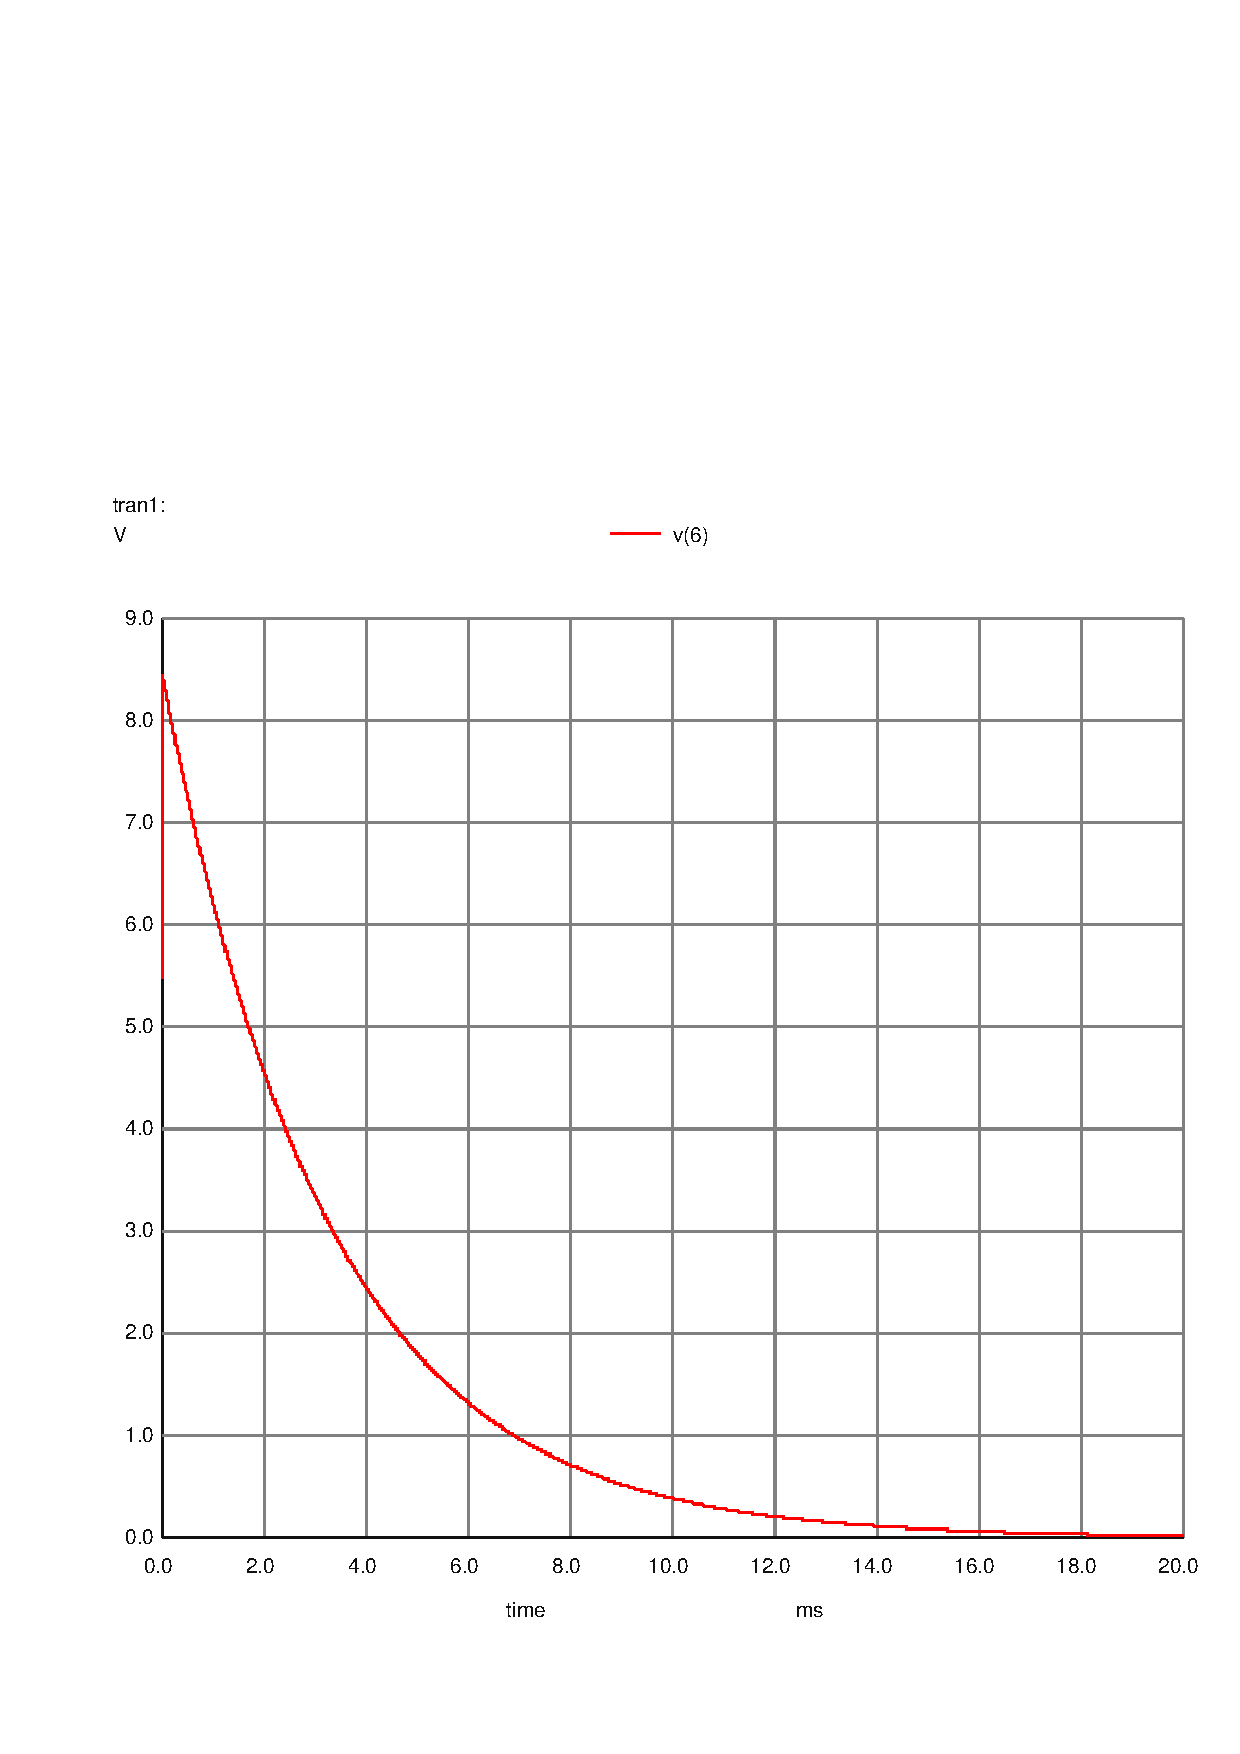
\includegraphics[width=0.6\linewidth, trim={2cm 1.5cm 0.5cm 6cm}, clip]{../Simulation/trans_nat.pdf}
    \caption{Natural response.}
    \label{fig:NatNg}
\end{figure}



\subsubsection{Transient analysis: Final solution}

\indent

After adding the normal and the complex solutions, the final solution is obtained, which can be seen in this graphic (Figure \ref{fig:ForNg}).

\begin{figure}[H] \centering
    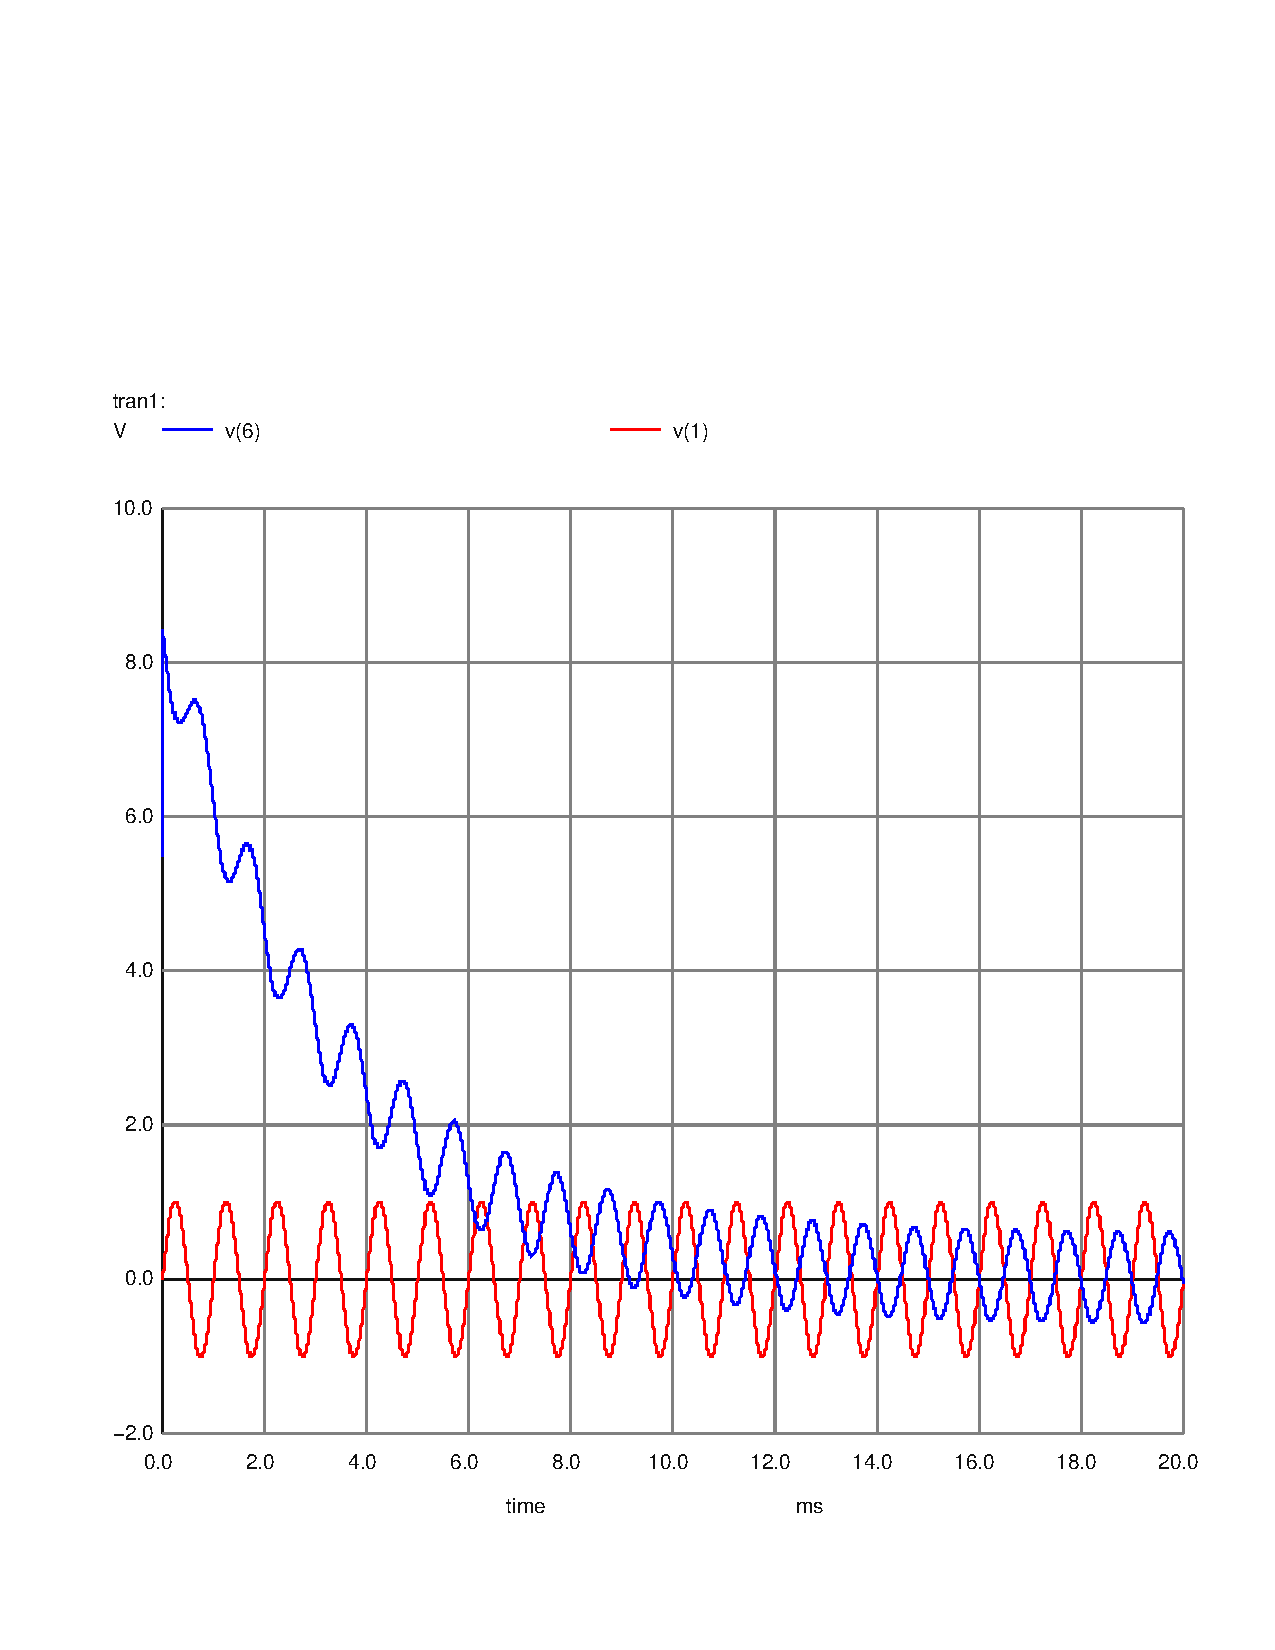
\includegraphics[width=0.6\linewidth, trim={2cm 1.5cm 0.5cm 6cm}, clip]{../Simulation/trans_forc.pdf}
    \caption{Forced response.}
    \label{fig:ForNg}
\end{figure}




\subsubsection{Frequency analysis}

\indent

When varying the frequency from 0,1 Hz to 1 MHz we get these graphics, which show how the magnitude (Figure \ref{fig:FreqMagNg} and \ref{fig:FreqMagDBNg}) and the phase (Figure \ref{fig:FreqPhNg}) vary with this change.

\begin{figure}[H] \centering
    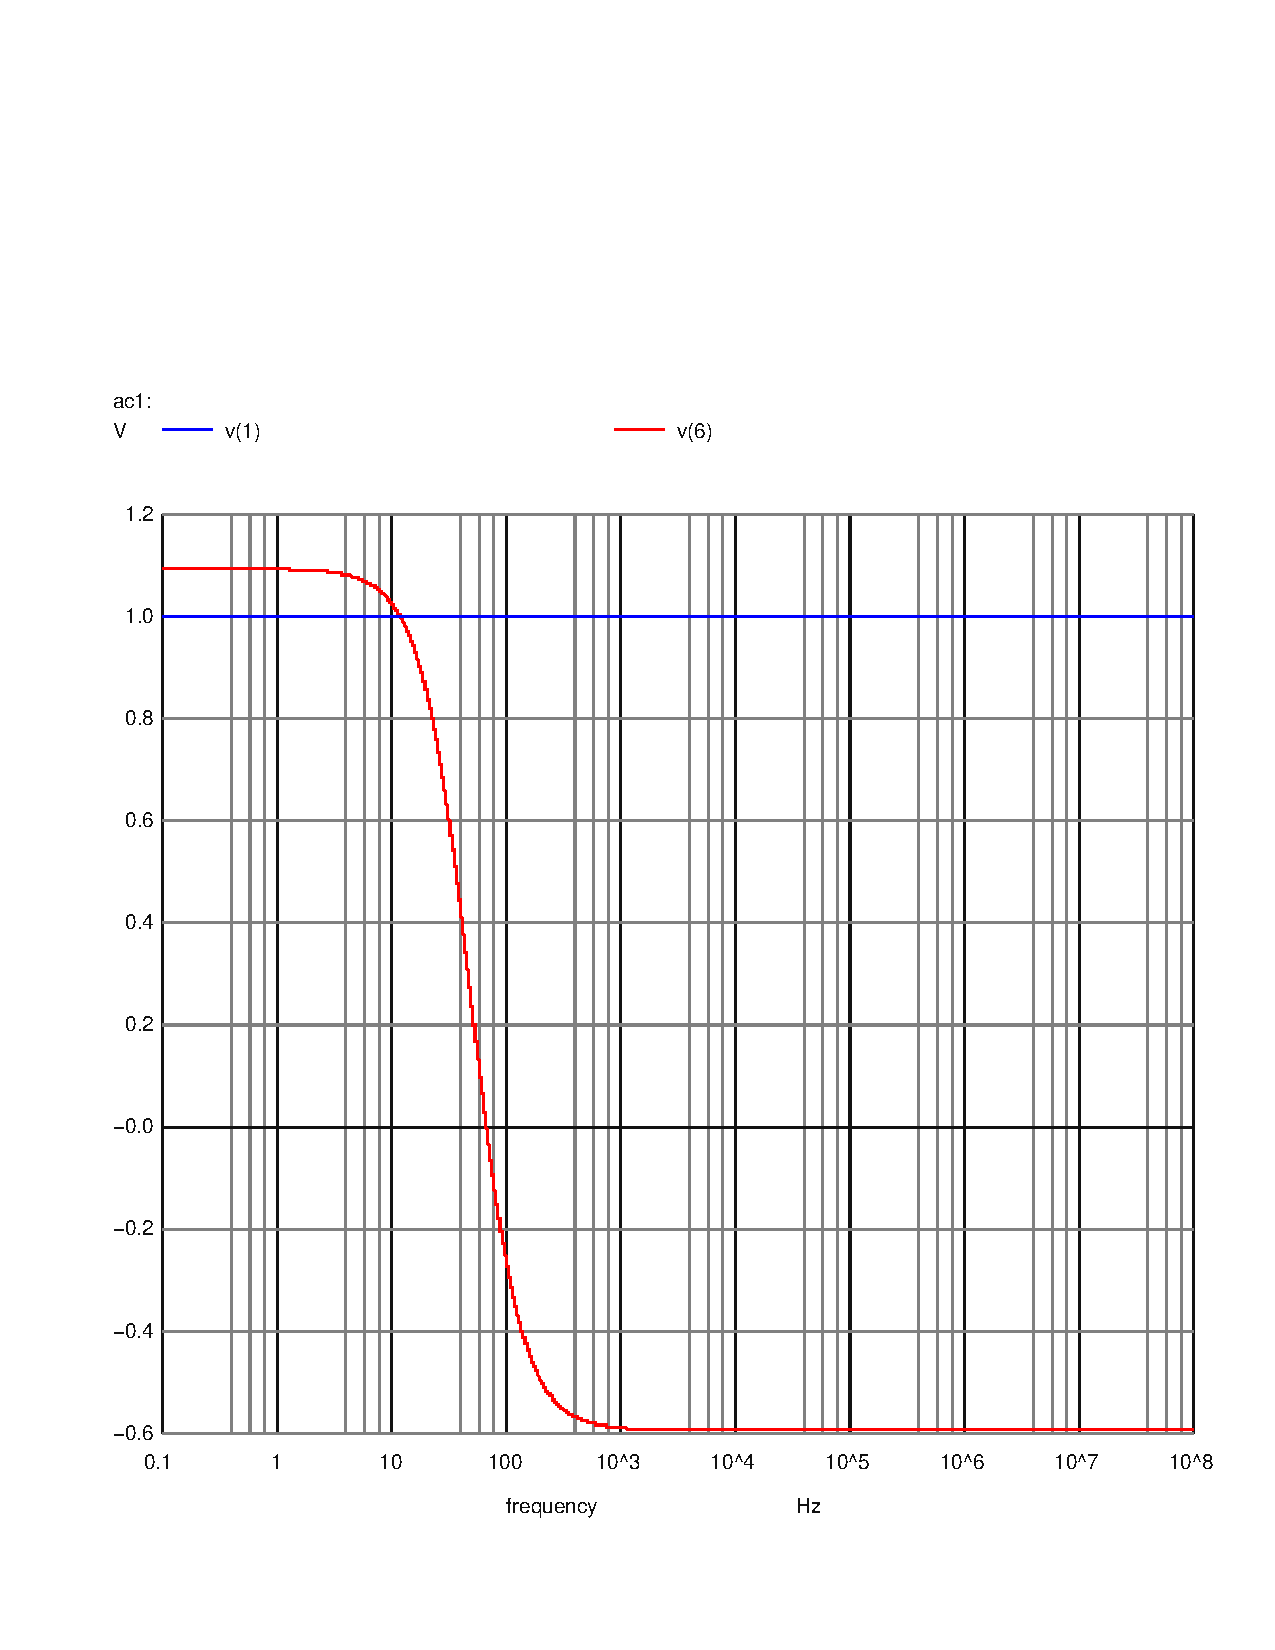
\includegraphics[width=0.6\linewidth, trim={2cm 1.5cm 0.5cm 6cm}, clip]{../Simulation/acm.pdf}
    \caption{Magnitude graph in volts.}
    \label{fig:FreqMagNg}
\end{figure}


\begin{figure}[H] \centering
    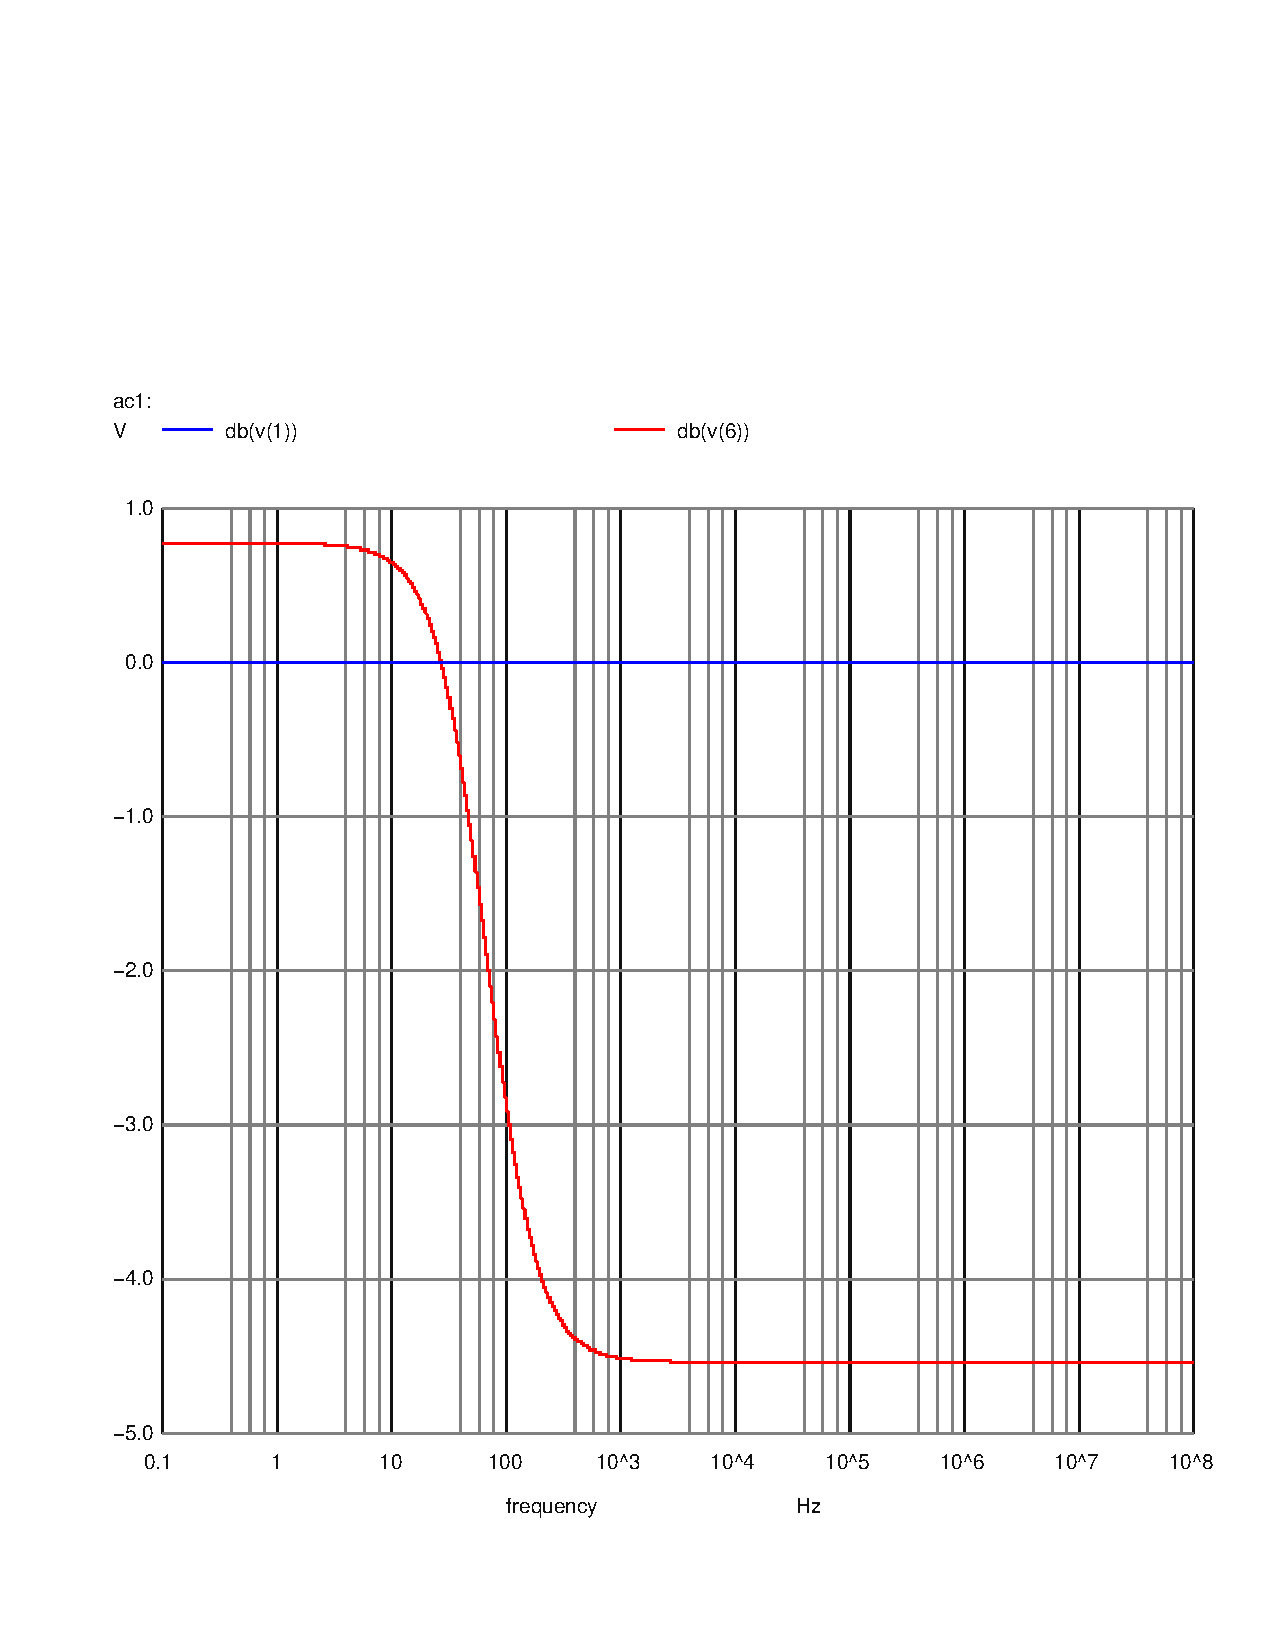
\includegraphics[width=0.6\linewidth, trim={2cm 1.5cm 0.5cm 6cm}, clip]{../Simulation/acm_db.pdf}
    \caption{Magnitude graph in dB.}
    \label{fig:FreqMagDBNg}
\end{figure}

\begin{figure}[H] \centering
    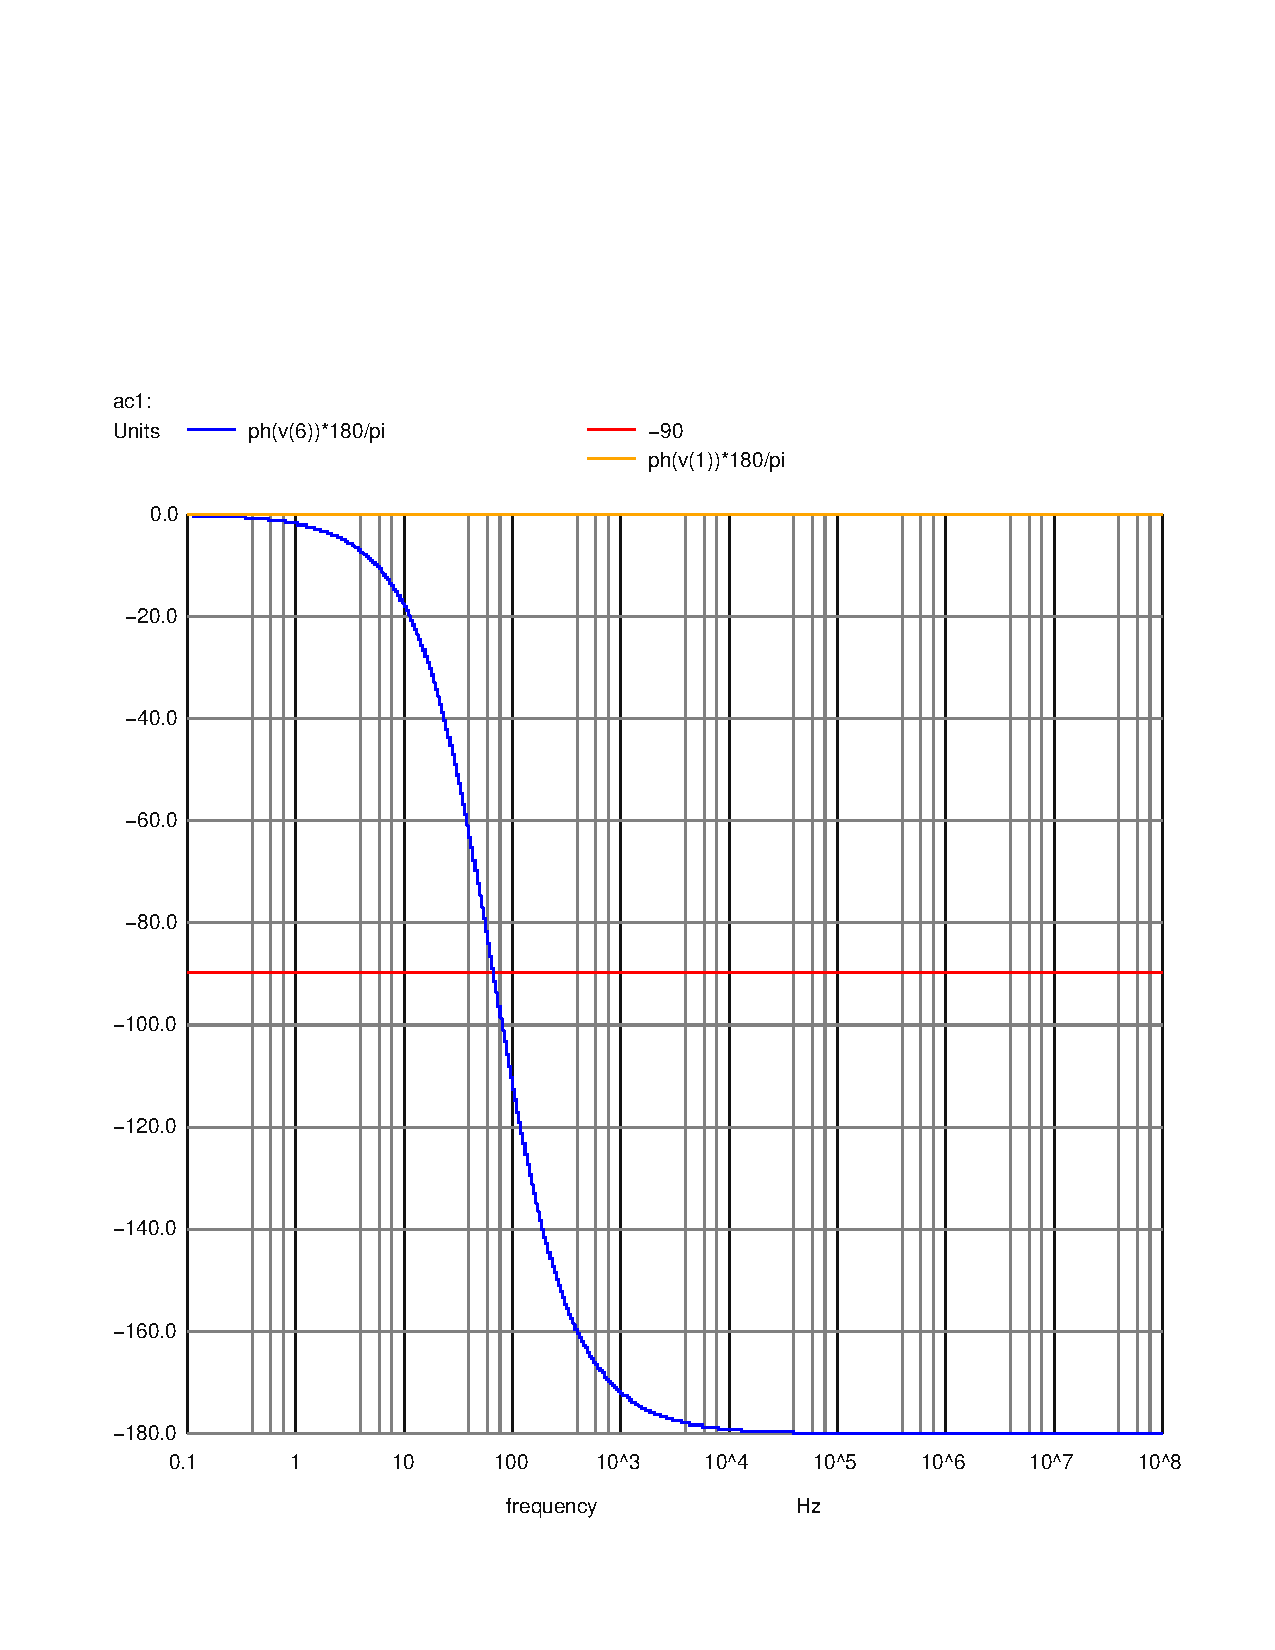
\includegraphics[width=0.6\linewidth, trim={2cm 1.5cm 0.5cm 6cm}, clip]{../Simulation/acph.pdf}
    \caption{Phase graph in degrees.}
    \label{fig:FreqPhNg}
\end{figure}
